\usetikzlibrary{calc}
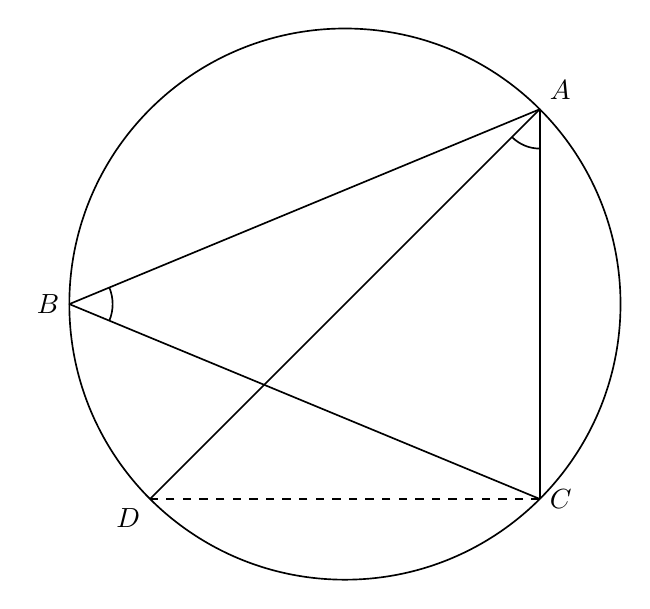
\begin{tikzpicture}[x=1cm,y=1cm,line width=.6pt,font=\normalsize]
\coordinate (O) at (0,0);
\coordinate (A) at (2.4749,2.4749);
\coordinate (B) at (-3.5,0);
\coordinate (C) at (2.4749,-2.4749);
\coordinate (D) at (-2.4749,-2.4749);
\draw[black] (O) circle[radius=3.5cm];
\draw[black] (A)--(B);
\draw[black] (B)--(C);
\draw[black] (A)--(C);
\draw[black] (A)--(D);
\draw[black,dashed] (C)--(D);
\draw[black] (B) ++(-22.5:0.55cm) arc[start angle=-22.5,end angle=22.5,radius=0.55cm];
\draw[black] (A) ++(-135:0.5cm) arc[start angle=-135,end angle=-90,radius=0.5cm];
\node[above right] at (A) {$A$};
\node[left] at (B) {$B$};
\node[right] at (C) {$C$};
\node[below left] at (D) {$D$};
\end{tikzpicture}
